%
% Artigo TCC II — Matheus Grassi Milanezi
% Sistema Inteligente de Apoio à Tomada de Decisão na Aviação Civil
% Versão 2 — artigo completo com sistema implementado e resultados
%
\documentclass[english,brazilian]{UNISINOSartigo}
\usepackage[utf8]{inputenc}
\usepackage[T1]{fontenc}
\usepackage{graphicx}
\usepackage{bibentry}
\usepackage{float}
\usepackage{array}
\usepackage{booktabs}
\usepackage{multirow}
\usepackage{newfloat}
\usepackage{setspace}

\usepackage[alf]{abntex2cite}

\newcolumntype{L}{>{\raggedright\arraybackslash}p{4.5cm}}
\newcolumntype{R}{>{\raggedright\arraybackslash}p{8.5cm}}
\newcolumntype{C}{>{\centering\arraybackslash}p{3cm}}
\newcolumntype{M}{>{\centering\arraybackslash}p{2.2cm}}

\autor{MILANEZI}{MATHEUS GRASSI}
\titulo{Sistema Inteligente de Apoio à Tomada de Decisão na Aviação Civil, baseado 
em Análise de Dados e Aprendizado de Máquina para Prevenção de Acidentes}
\subtitulo{}
\orientador[Prof.~Dr.]{Kunst}{Rafael}
\local{Porto Alegre}
\ano{2026}
\unidade{Unidade Acadêmica de Graduação}
\curso{Curso de Bacharelado em Ciência da Computação}
\natureza{%
Artigo apresentado como requisito parcial para obtenção do título de
Bacharel em Ciência da Computação, pelo Curso de Ciência da Computação da
Universidade do Vale do Rio dos Sinos (UNISINOS)}

\begin{document}
\capa
\folhaderosto

\tituloArtigo{Sistema Inteligente de Apoio à Tomada de Decisão na Aviação Civil,
baseado em Análise de Dados e Aprendizado de Máquina para Prevenção de Acidentes}{%
}

\autorArtigo{Matheus Grassi Milanezi\footnote{Graduando do curso de Bacharelado em
Ciências da Computação da Universidade do Vale do Rio dos Sinos (UNISINOS).
E-mail: mmilanezi@edu.unisinos.br}}

\autorArtigo{Rafael Kunst\footnote{Orientador. Professor Dr. do curso de Ciências
da Computação da Universidade do Vale do Rio dos Sinos (UNISINOS).
E-mail: rafaelkunst@unisinos.br}}

%=======================================================================
\begin{abstract}
A segurança operacional na aviação civil enfrenta um desafio crescente: à medida
que os índices de acidentes diminuem, torna-se mais difícil identificar riscos ocultos
antes que se materializem em eventos adversos. Este trabalho apresenta o
desenvolvimento de um Sistema Inteligente de Apoio à Decisão Pré-Voo que combina
dados históricos de ocorrências da aviação civil brasileira (CENIPA, 2007--2025),
variáveis meteorológicas obtidas do INMET e da API Open-Meteo, além de
características da aeronave e do itinerário, para classificar automaticamente o risco
de cada etapa de um voo. O modelo preditivo é baseado em um Stacking Ensemble
composto por quatro algoritmos de aprendizado de máquina supervisionado,
Random Forest, XGBoost, SVM-RBF e Perceptron Multicamadas (MLP),
combinados por uma Regressão Logística Multinomial como meta-aprendiz. O
balanceamento de classes foi realizado via SMOTE e a geração de dados sintéticos
para representar voos normais, enquanto a validação empregou predições
\textit{out-of-fold} com validação cruzada de 5 partições. O modelo alcançou
acurácia de 87,54\%, F1-Score Macro de 74,28\% e ROC-AUC de 95,07\% no conjunto
de teste, classificando operações aéreas em quatro categorias: Apto Seguro,
Apto Requer Atenção, Não Apto e Inconclusivo. O sistema integra uma interface web com
consulta meteorológica em tempo real, \textit{overrides} automáticos de segurança
e geração de relatório em PDF, constituindo uma ferramenta prática alinhada ao
paradigma Safety-II para o planejamento pré-voo na aviação civil brasileira.

\palavraschave{Aviação civil. Segurança operacional. Aprendizado de máquina.
Análise pré-voo. Stacking Ensemble. Inteligência artificial.}
\end{abstract}

\begin{otherlanguage}{english}
\singlespacing
\begin{abstract}
Civil aviation operational safety faces a growing challenge: as accident rates decline,
identifying latent risks before they materialize into adverse events becomes
increasingly difficult. This paper presents the development of an Intelligent Pre-Flight
Decision Support System that combines historical records of Brazilian civil aviation
occurrences (CENIPA, 2007--2025), meteorological data from INMET and the
Open-Meteo API, and aircraft and itinerary characteristics to automatically classify the
risk of each flight segment. The predictive model is based on a Stacking Ensemble of
four supervised machine learning algorithms , Random Forest, XGBoost, SVM-RBF,
and Multilayer Perceptron (MLP) , combined by a Multinomial Logistic Regression
meta-learner. Class balancing was performed via SMOTE and synthetic data generation
for normal flight representation, while validation employed out-of-fold predictions with
5-fold cross-validation. The model achieved 87.54\% accuracy, 74.28\% F1 Macro Score,
and 95.07\% ROC-AUC on the test set, classifying flight operations into four
operational categories: Safe, Requires Attention, Not Apt, and Inconclusive. The system integrates a web
interface with real-time meteorological queries, automatic safety overrides, and PDF
report generation, constituting a practical tool aligned with the Safety-II paradigm for
pre-flight planning in Brazilian civil aviation.
\end{abstract}
\palavraschave{Civil aviation. Operational safety. Machine learning. Pre-flight
analysis. Stacking Ensemble. Artificial intelligence.}
\end{otherlanguage}

%=======================================================================
\section{Introdução}
%=======================================================================

A aviação civil consolidou-se, ao longo das últimas décadas, como um dos meios
de transporte mais seguros do mundo graças ao avanço contínuo de tecnologias,
práticas de gerenciamento de risco e sistemas regulatórios rigorosos. Entretanto,
a crescente complexidade das operações, influenciada por variabilidade
meteorológica, pressões operacionais, diversidade de aeronaves e aumento do
tráfego, impõe novos desafios à manutenção da segurança operacional. Nesse
contexto, o planejamento pré-voo torna-se uma etapa fundamental, pois permite a
identificação antecipada de condições que podem comprometer a operação e a
adoção de medidas preventivas antes que tais riscos se manifestem em voo.

Ferramentas tradicionais de avaliação de risco pré-voo, como o \textit{Flight
Risk Assessment Tool} (FRAT), desempenham papel importante, mas apresentam
limitações reconhecidas na literatura. \citeonline{WALDEN2023} destacam que esses
instrumentos dependem fortemente de entradas manuais, sofrem influência do viés
humano e não integram automaticamente variáveis meteorológicas, históricas e
operacionais, o que reduz a sensibilidade da análise em cenários dinâmicos.
Modelos de \textit{Machine Learning} surgem como alternativa para fornecer uma
categorização de risco mais consistente e menos subjetiva.

Paralelamente, a evolução recente da Inteligência Artificial (IA) demonstrou grande
potencial para fortalecer os sistemas de segurança aeronáutica. A revisão
sistemática de \citeonline{DEMIR2024}, abrangendo 224 estudos publicados entre
2004 e 2024, evidencia crescimento expressivo na aplicação de ML, aprendizado
profundo e modelos de séries temporais à análise de acidentes, previsão de eventos
de risco e melhoria das medidas de segurança. Entretanto, cada estudo tende a
abordar apenas um aspecto isolado da operação, seja clima, manutenção ou dados
históricos , sem propor uma estrutura verdadeiramente integrada. Nesse cenário,
\citeonline{ZIAKKAS2024} situam a IA como elemento central na transição do
paradigma \textit{Safety-I} , reativo, centrado na investigação de falhas , para o
\textit{Safety-II}, que busca compreender por que operações dão certo,
fortalecendo a resiliência sistêmica.

Diante desse panorama, identificou-se uma lacuna relevante: a ausência de
ferramentas que consolidem múltiplas dimensões do risco pré-voo , meteorológica,
operacional, histórica e de rota , em uma única análise automatizada. Este trabalho
descreve o desenvolvimento e a avaliação de um sistema inteligente de apoio à
tomada de decisão pré-voo, que combina dados históricos do CENIPA
\cite{CENIPA2024}, variáveis meteorológicas reais e características da aeronave e
do itinerário para estimar automaticamente o nível de risco associado a cada ponto
de uma operação aérea, utilizando um modelo de Stacking Ensemble supervisionado.

O sistema desenvolvido alcançou acurácia de 87,54\%, F1-Score Macro de 0,7428
e ROC-AUC de 0,9507, classificando operações aéreas em quatro categorias
operacionais. Além do modelo preditivo, foi implementada uma interface web com
consulta meteorológica em tempo real, lógica de \textit{overrides} de segurança e
geração de relatório técnico em PDF. O trabalho busca, assim, contribuir para a
evolução das práticas de segurança operacional na aviação civil brasileira, oferecendo
uma abordagem integrada, orientada por dados e alinhada ao paradigma
\textit{Safety-II}.

%=======================================================================
\section{Fundamentação Teórica}
%=======================================================================

A presente seção apresenta os fundamentos teóricos que sustentam o
desenvolvimento deste trabalho, abrangendo a evolução da segurança operacional
na aviação, os conceitos de avaliação de risco pré-voo, a importância dos dados
históricos e as técnicas de Inteligência Artificial e Aprendizado de Máquina
aplicadas ao contexto aeronáutico.

\subsection{História e evolução da segurança operacional na aviação civil}

A segurança operacional constitui um dos pilares centrais da aviação civil desde
o surgimento do transporte aéreo comercial. Ao longo das décadas, a compreensão
sobre como prevenir acidentes evoluiu profundamente, impulsionada por avanços
tecnológicos, debates conceituais e pelo aumento da complexidade das operações
aéreas. Como destaca \citeonline{HARMS2020}, a trajetória da segurança pode ser
entendida pela mudança de foco entre três grandes grupos de fatores: técnicos,
humanos e organizacionais/sistêmicos.

Nas primeiras décadas da aviação comercial, especialmente entre os anos 1950
e 1970, a maioria dos acidentes era atribuída a falhas técnicas, estruturais ou de
projeto. Consequentemente, os esforços de segurança se concentravam quase que
exclusivamente na melhoria do desempenho mecânico, na padronização de
procedimentos de manutenção, na certificação de aeronaves e no fortalecimento da
confiabilidade dos equipamentos. Com o amadurecimento tecnológico e a redução
das falhas mecânicas, o setor identificou o erro humano como o principal fator
contribuinte para acidentes, deslocando a atenção para treinamento, ergonomia,
fatores cognitivos e cultura organizacional.

A partir da década de 1990, consolidou-se um novo entendimento: o acidente
não é resultado de um único erro humano, mas sim o produto de falhas sucessivas
dentro de um sistema complexo. Nesse período, como enfatiza \citeonline{HARMS2020},
reconheceu-se que as condições organizacionais, pressões operacionais, limitações
do ambiente e processos internos influenciavam o desempenho humano. Essa
mudança marcou o início de uma transição conceitual e prática, de um modelo
essencialmente reativo para um modelo progressivamente proativo e preditivo.

Esse movimento foi formalizado no contraste entre \textit{Safety-I} e
\textit{Safety-II}, conforme discutem \citeonline{ZIAKKAS2024}. O \textit{Safety-I}
define segurança como a ausência de falhas e atua de forma reativa, investigando o
que deu errado após sua ocorrência. Já o \textit{Safety-II} entende segurança como
a capacidade de garantir que ``as coisas deem certo'', enfatizando adaptação,
resiliência e antecipação de riscos. Essa visão ampliada está diretamente associada
à evolução dos Sistemas de Gerenciamento da Segurança Operacional (SMS), que
incorporam práticas de monitoramento contínuo, identificação precoce de ameaças e
mitigação proativa.

Nesse contexto, \citeonline{ZIEJA2015} mostram que os sistemas de informação
passaram a desempenhar papel fundamental nessa nova abordagem. O uso de bases
de dados, métodos estatísticos e ferramentas de análise permite identificar
correlações entre incidentes e acidentes, detectar tendências de falhas e
compreender padrões operacionais, baseando a tomada de decisão em evidências e
indicadores. Paralelamente, como observa \citeonline{HARMS2020}, a aviação atingiu
níveis tão elevados de segurança que acidentes tornaram-se eventos raros, o que
desafia os métodos tradicionais de vigilância e exige novas formas de análise
capazes de revelar riscos ocultos. Diante disso, o avanço para um modelo
plenamente proativo e preditivo aponta naturalmente para o uso de técnicas de
Inteligência Artificial e Aprendizado de Máquina, alinhado ao paradigma
\textit{Safety-II}.

\subsection{Avaliação de risco e o conceito de análise pré-voo}

A avaliação de risco pré-voo constitui uma das etapas mais relevantes do
gerenciamento da segurança operacional, pois permite identificar perigos, avaliar a
exposição ao risco e adotar medidas de mitigação antes da decolagem. Ferramentas
como o \textit{Flight Risk Assessment Tool} (FRAT) foram desenvolvidas para
estruturar esse processo, mensurando o nível de risco associado a uma operação
aérea antes que ela ocorra. Esses instrumentos utilizam questionários e pontuações
baseadas em fatores como condições meteorológicas, experiência e proficiência do
piloto, características da aeronave, manutenção, familiaridade com o aeródromo e
perfil da missão.

Como apresentado por \citeonline{WALDEN2023}, durante o planejamento pré-voo
o piloto deve considerar múltiplos elementos antes de decidir se irá voar, devendo
analisar utilizando ferramentas como o FRAT. Essa análise sistemática também é
reforçada por \textit{checklists} como o PAVE , acrônimo de \textit{Pilot,
Aircraft, enVironment} e \textit{External Pressures} , que orienta o piloto a avaliar
os principais itens de risco.

Apesar de amplamente utilizados, estudos recentes apontam limitações
significativas no FRAT tradicional. Essas ferramentas dependem de entradas manuais
e da interpretação subjetiva do operador, o que pode gerar inconsistências, vieses
cognitivos e subestimação de riscos \cite{WALDEN2023}. Além disso, os modelos
atuais não integram dados históricos de acidentes, relatórios de incidentes ou
análises automatizadas, reduzindo sua precisão e abrangência. \citeonline{WALDEN2023}
destacam que muitos FRATs apresentam baixa acessibilidade, questionários
incompletos, elevado tempo de preenchimento e ausência de requisitos regulatórios
que incentivem seu uso contínuo, além de não incorporar a probabilidade de
ocorrência dos perigos.

Buscando superar essas limitações, \citeonline{WALDEN2023} propõem a
modernização do FRAT por meio de modelos de aprendizado de máquina treinados
com bases históricas de mais de 40 anos de registros do \textit{National
Transportation Safety Board} (NTSB). \citeonline{FELDMAN2023} complementam ao
descrever o \textit{In-Time Aviation Safety Management System} (IASMS) da NASA,
que reúne dados de múltiplas fontes aeronáuticas e ambientais para gerar
diagnósticos preditivos durante o planejamento, demonstrando que a automação
aumenta a consciência situacional do operador.

Outro aspecto crítico diz respeito à meteorologia. \citeonline{LIU2024} ressaltam que
fenômenos como turbulência severa, \textit{windshear}, tempestades convectivas e
baixa visibilidade impactam diretamente a segurança operacional, e que a melhoria
da capacidade de alerta antecipado de tempo severo é uma das principais funções
dos serviços de meteorologia aeronáutica. Essa compreensão reforça que muitos
acidentes têm origem ainda na fase de preparação: de acordo com Wright
(2019, \textit{apud} \citeauthor{WALDEN2023}, \citeyear{WALDEN2023}), falhas de
gestão de risco foram causa raiz de quase 50\% dos acidentes fatais com aeronaves
de negócios, e a maioria poderia ser rastreada a deficiências no planejamento
pré-voo.

\subsection{A importância dos dados de voo e relatórios de incidentes}

Os dados de voo, os registros de manutenção e os relatórios de incidentes
constituem a base da gestão moderna da segurança operacional. \citeonline{DEMIR2024}
destacam que a análise sistemática de conjuntos massivos de dados permite
identificar padrões de risco, detectar anomalias operacionais e aprimorar a
capacidade preditiva dos modelos de segurança. \citeonline{ZIEJA2015} reforçam o
papel dos sistemas de informação na identificação de relações entre variáveis
críticas , falhas técnicas, fatores humanos e condições operacionais , orientando
decisões mais precisas por meio de análise de padrões recorrentes e possíveis
relações causais.

O uso contínuo desses registros não apenas sustenta avaliações de desempenho
e auditorias de segurança, mas também possibilita o desenvolvimento de relatórios
estatísticos e indicadores que medem a eficácia de programas de treinamento e
ações mitigadoras. Conforme afirmam \citeonline{DEMIR2024}, modelos baseados em
IA dependem de dados históricos de voo, registros de manutenção e relatórios de
incidentes para aprender continuamente com as ocorrências operacionais e produzir
previsões confiáveis. \citeonline{HARMS2020} enfatiza que a segurança na aviação
está cada vez mais associada à análise automatizada de dados, cujo impacto na
avaliação do desempenho de segurança operacional torna-se crescentemente
determinante.

Nesse contexto, os dados tornam-se elementos estruturantes da segurança
operacional. Sem bases de dados consistentes, extensas e confiáveis, não há como
desenvolver modelos preditivos robustos, identificar precursores de risco ou
sustentar práticas proativas alinhadas ao paradigma \textit{Safety-II}.
A gestão de dados emerge, portanto, como componente essencial para qualquer
iniciativa de IA aplicada à segurança de voo.

\subsection{Inteligência artificial e aprendizado de máquina aplicados à segurança
aeronáutica}

O desenvolvimento de sistemas inteligentes de apoio à tomada de decisão na
aviação civil insere-se em um movimento global de transição do paradigma
\textit{Safety-I} para o \textit{Safety-II}, voltado à compreensão de por que as
operações aéreas são bem-sucedidas e ao fortalecimento da resiliência sistêmica
\cite{ZIAKKAS2024}. Nesse contexto, \citeonline{KUHL2022} distinguem Inteligência
Artificial (IA) de Aprendizado de Máquina (ML): IA é o campo mais amplo voltado
ao desenvolvimento de agentes capazes de perceber e agir racionalmente, enquanto
o ML constitui o subconjunto de métodos que permitem ao sistema aprender padrões
a partir de dados, sem que regras sejam explicitamente programadas. A convergência
dessas tecnologias com a aviação é documentada por \citeonline{DEMIR2024}, cuja
revisão sistemática de 224 estudos publicados entre 2004 e 2024 evidencia
crescimento expressivo na aplicação de ML à análise de acidentes, previsão de
eventos de risco e melhoria das medidas de segurança operacional.

A aviação moderna tornou-se um terreno fértil para soluções baseadas em dados,
pois combina um sistema de altíssimo nível de segurança com uma infraestrutura de
registro detalhado de eventos, falhas, condições meteorológicas e parâmetros
operacionais. Esse ambiente fornece o que algoritmos de ML mais precisam: grandes
volumes de dados estruturados, contínuos e historicamente ricos.

\subsubsection{Fundamentos do aprendizado supervisionado no contexto da aviação}

Dentro do campo do ML, o aprendizado supervisionado é a categoria que mais
se destaca nas aplicações aeronáuticas. Segundo \citeonline{MITCHELL1997}, um
programa aprende a partir de uma experiência de treino com respeito a uma tarefa e
uma medida de desempenho se seu desempenho na tarefa, medido por essa métrica,
melhora com a experiência fornecida , definição que captura o processo pelo qual
os modelos preditivos aprendem a estimar o risco de voo a partir de ocorrências
históricas rotuladas. \citeonline{KUHL2022} complementam que esses modelos
``aprendem'' relações internas nos dados e ajustam seu comportamento com base
nessa experiência, em vez de dependerem apenas de instruções pré-programadas.

No presente trabalho, cada registro do banco de dados do CENIPA \cite{CENIPA2024}
foi associado a um rótulo de gravidade: Voo Normal (Classe~0), Incidente
(Classe~1), Incidente Grave (Classe~2) ou Acidente (Classe~3), fornecendo ao
modelo a experiência de treinamento necessária para generalizar o padrão de risco
a novos voos não observados. Na prática da aviação, esse paradigma é aplicado para
identificar se um voo representa risco baixo ou elevado, prever se condições
meteorológicas são perigosas e antecipar precursores de acidentes, encaixando-se
diretamente no modelo supervisionado porque envolvem padrões já observados
em eventos passados e rotulagem operacional compatível.

\subsubsection{Modelos de aprendizado de máquina utilizados}

Para a composição dos modelos base do ensemble, foram selecionados quatro
algoritmos de naturezas distintas, escolha motivada pela necessidade de diversidade
entre os preditores, conforme preconizado por \citeonline{HASTIE2009}.

O primeiro modelo base é o \textbf{Random Forest} (RF), descrito por
\citeonline{HASTIE2009} como uma variação substancial do \textit{bagging} que
constrói uma coleção de árvores descorrelacionadas e combina suas predições por
voto majoritário, atingindo desempenho comparável ao \textit{boosting} com menor
custo de ajuste. \citeonline{GERON2019} complementa que o algoritmo introduz
aleatoriedade adicional na seleção de variáveis em cada nó da árvore, reduzindo a
variância sem aumentar proporcionalmente o viés , propriedade especialmente
valiosa em dados aeronáuticos heterogêneos e ruidosos. \citeonline{WALDEN2023}
confirmam sua eficácia no contexto aeronáutico, apontando o Random Forest como
um dos dois modelos de melhor desempenho dentre XGBoost, RF, redes neurais e
BERT para categorização de risco pré-voo.

O segundo modelo base é o \textbf{XGBoost} (\textit{Extreme Gradient Boosting}),
implementação otimizada do Gradient Boosting fundamentado matematicamente por
\citeonline{HASTIE2009} como a minimização de uma função de perda no espaço
funcional por meio de gradiente descendente. \citeonline{GERON2019} reconhece o
XGBoost como componente frequente nas soluções vencedoras de competições de
aprendizado de máquina, graças à sua capacidade de capturar interações complexas
entre variáveis operacionais e meteorológicas aliada à relativa interpretabilidade via
importância de \textit{features}. \citeonline{WALDEN2023} adotaram o modelo como
referência central na modernização do FRAT.

O terceiro modelo base é a \textbf{Máquina de Vetores de Suporte com kernel de
função de base radial} (SVM-RBF), especialmente indicada quando as fronteiras de
decisão entre classes são complexas e não-lineares, situação frequente em dados
operacionais aeronáuticos. Segundo \citeonline{HASTIE2009} e \citeonline{GERON2019},
o kernel RBF projeta os dados em um espaço de características de alta dimensão
onde a separação linear se torna viável, conferindo ao modelo grande flexibilidade
sem requerer transformações manuais das variáveis. No presente trabalho, o
SVM-RBF atua como um dos preditores base do ensemble, processando as variáveis
meteorológicas e operacionais do itinerário. A eficácia do SVM em contextos
aeronáuticos com variáveis similares é evidenciada por \citeonline{LIU2024}, que
aplicaram SVM-RBF para a tarefa específica de previsão de condições meteorológicas
perigosas , tempestades, turbulência e baixa visibilidade , obtendo desempenho
superior ao de Random Forest e LSTM em acurácia, ROC-AUC e F1-score.

O quarto modelo base é o \textbf{Perceptron Multicamadas} (MLP), uma rede neural
artificial do tipo \textit{feedforward} treinada por retropropagação do gradiente,
cuja arquitetura com camadas ocultas e função de ativação não-linear permite
aprender representações hierárquicas dos dados \cite{HASTIE2009,MITCHELL1997}.
\citeonline{HARMS2020} demonstra, em contexto aeronáutico real, que redes MLP
com otimizador Adam, ativação ReLU e \textit{early stopping} são capazes de
identificar precursores indiretos de eventos de segurança de voo, com os parâmetros
meteorológicos ocupando posição dominante no ranking de relevância de
\textit{features} atribuído pelo algoritmo Relief. No presente trabalho, o MLP foi
configurado com uma camada oculta e otimizador Adam, atuando como complemento
não-linear dos demais modelos base.

\subsubsection{Stacking Generalizado como técnica de combinação de modelos}

A combinação dos quatro modelos base foi realizada pela técnica de
\textbf{Stacking Generalizado}, proposta originalmente por \citeonline{WOLPERT1992}.
O Stacking é uma abordagem de combinação de modelos (\textit{ensemble}) em que,
ao invés de se escolher um único melhor modelo ou combinar predições por média
simples, os modelos base , chamados de \textit{nível 0} ou \textit{base
learners} , são treinados de forma independente e suas predições são utilizadas
como entrada de um novo modelo, o meta-aprendiz de \textit{nível 1}, que aprende
qual combinação entre eles produz o melhor resultado global.
\citeonline{HASTIE2009} formalizam que a combinação de modelos nunca piora o
desempenho esperado em relação a qualquer modelo individual quando estimada no
nível populacional, fundamentando a utilização de ensembles em tarefas de
classificação complexas.

Para garantir que as predições utilizadas no treinamento do meta-aprendiz fossem
não enviesadas, utilizou-se a técnica de \textbf{predições out-of-fold} com
\textbf{validação cruzada de 5 partições} (\textit{5-fold cross-validation}). Nessa
abordagem, o conjunto de treinamento é dividido em 5 subconjuntos (\textit{folds})
de tamanho aproximadamente igual. Para cada \textit{fold}, os modelos base são
treinados nos 4 subconjuntos restantes e geram predições para o subconjunto
reservado, de modo que ao final do processo cada instância de treinamento possui
uma predição gerada por um modelo que nunca a viu durante o treino. Essas
predições fora da amostra são chamadas de \textit{out-of-fold predictions} e
constituem as \textit{meta-features} que alimentam o meta-aprendiz.
\citeonline{GERON2019} reforça que esse procedimento assegura que as predições
são limpas, uma vez que os preditores de nível zero nunca treinaram sobre as
instâncias reservadas. \citeonline{WALDEN2023} adotam procedimento equivalente
de validação cruzada para garantir a generalização dos modelos de FRAT
modernizado.

Como meta-aprendiz de \textit{nível 1}, foi adotada a \textbf{Regressão Logística
Multinomial com regularização L2} (C\,=\,1,0). A escolha por um modelo linear como
combinador é fundamentada por \citeonline{WOLPERT1992} e \citeonline{HASTIE2009},
que recomendam modelos simples nesse papel porque o espaço de meta-features já
contém a informação discriminativa destilada pelos modelos de nível 0, e modelos
mais simples tendem a generalizar melhor nessa posição, evitando
\textit{overfitting} do meta-nível.

\subsubsection{Aplicações da IA na segurança aeronáutica e limitações identificadas
pela literatura}

A literatura recente revela que a IA tem desempenhado papéis diversos e
complementares na segurança aeronáutica, mas também evidencia limitações
estruturais que ainda impedem a formação de sistemas verdadeiramente integrados.
\citeonline{HARMS2020} demonstra que técnicas supervisionadas são capazes de
prever eventos de segurança com base em variáveis indiretas, mas destaca que a
eficácia dos modelos depende fortemente da disponibilidade de dados históricos,
especialmente porque eventos negativos são raros , desafio que o presente
trabalho aborda por meio da geração de dados sintéticos e do balanceamento via
SMOTE.

\citeonline{WALDEN2023} evidenciam que modelos como XGBoost, Random Forest,
redes neurais e BERT melhoram a consistência e precisão do processo de avaliação
de risco pré-voo, mas observam que ferramentas atuais geralmente não integram
dados meteorológicos, operacionais e históricos de maneira conjunta. A revisão
sistemática de \citeonline{DEMIR2024} reforça esse cenário ao apontar que grande
parte das pesquisas aplica IA a fatores isolados da operação aérea, sem propor um
modelo unificado.

Por fim, \citeonline{ZIAKKAS2024} situam a IA como elemento essencial do
paradigma \textit{Safety-II}, mas reforçam que a eficácia desses sistemas depende
da integração de informações diversas e de interfaces claras , algo que o presente
trabalho buscou concretizar ao reunir dados de múltiplas fontes em um único
sistema funcional voltado ao operador aéreo.

%=======================================================================
\section{Desenvolvimento do Sistema}
%=======================================================================

O sistema desenvolvido é uma aplicação web de apoio à decisão pré-voo que
integra dados históricos, meteorológicos e operacionais para classificar
automaticamente o nível de risco de cada ponto de um itinerário aéreo. A
arquitetura é organizada em quatro camadas funcionais: \textbf{dados},
\textbf{processamento}, \textbf{inferência} e \textbf{apresentação}.

A camada de dados reúne as fontes brutas: os arquivos históricos do CENIPA
\cite{CENIPA2024} (ocorrências 2006--2023), os arquivos CSV do INMET
\cite{INMET2024} organizados por ano e estado (2000--2026) e a base pública de
aeródromos brasileiros do OurAirports. A camada de processamento engloba os
scripts de ingestão, integração, geração de dados sintéticos e engenharia de
\textit{features}. A camada de inferência carrega o modelo Stacking Ensemble
serializado e aplica a lógica de status e \textit{overrides} de segurança. Por fim,
a camada de apresentação disponibiliza uma interface web via Flask, com geração
de relatório técnico em PDF pela biblioteca ReportLab e consulta meteorológica em
tempo real à API Open-Meteo para datas futuras.

\subsection{Engenharia de features}

O vetor de entrada do modelo é composto por 25 \textit{features} brutas que, após
pré-processamento, expandem-se para 189 dimensões. As 13 \textit{features}
numéricas são submetidas ao StandardScaler; as 12 \textit{features} binárias são
utilizadas sem transformação; e as 5 \textit{features} categóricas são codificadas
pelo OneHotEncoder, gerando aproximadamente 164 colunas adicionais. O
Quadro~\ref{quad:features} apresenta as variáveis numéricas e binárias do modelo.

\begin{quadro}[ht]
  \caption{Features numéricas e binárias do modelo preditivo}
  \label{quad:features}
  \centering
  \begin{tabular}{lp{7cm}}
    \toprule
    \textbf{Feature} & \textbf{Descrição} \\
    \midrule
    \multicolumn{2}{l}{\textit{Numéricas (StandardScaler)}} \\
    \texttt{pave\_vento\_ms}       & Velocidade do vento (m/s) \\
    \texttt{pave\_rajada\_ms}      & Velocidade da rajada (m/s) \\
    \texttt{pave\_precipitacao\_mm}& Precipitação (mm) \\
    \texttt{pave\_umidade\_pct}    & Umidade relativa (\%) \\
    \texttt{pave\_temp\_c}         & Temperatura (°C) \\
    \texttt{pave\_pressao\_mb}     & Pressão atmosférica (mb) \\
    \texttt{pave\_hora\_voo}       & Hora do voo (0--23) \\
    \texttt{pave\_mes}             & Mês do voo (1--12) \\
    \texttt{pave\_num\_motores}    & Quantidade de motores \\
    \texttt{pave\_pmd\_kg}         & Peso máximo de decolagem (kg) \\
    \texttt{pave\_idade\_aeronave} & Idade da aeronave (anos) \\
    \texttt{pave\_aeronave\_assentos} & Número de assentos \\
    \texttt{pave\_n\_tipos}        & N.º de tipos de ocorrência associados \\
    \midrule
    \multicolumn{2}{l}{\textit{Binárias (sem transformação)}} \\
    \texttt{pave\_vento\_forte}    & Vento $>$ 10 m/s (1/0) \\
    \texttt{pave\_rajada\_forte}   & Rajada $>$ 15 m/s (1/0) \\
    \texttt{pave\_chuva}           & Precipitação $>$ 1 mm (1/0) \\
    \texttt{pave\_umidade\_alta}   & Umidade $>$ 90\% (1/0) \\
    \texttt{pave\_voo\_noturno}    & Horário noturno, 20h--6h (1/0) \\
    \texttt{pave\_fase\_critica}   & Fase crítica: decolagem ou pouso (1/0) \\
    \texttt{pave\_fase\_solo}      & Fase em solo: táxi (1/0) \\
    \texttt{pave\_instrucao}       & Voo de instrução (1/0) \\
    \texttt{pave\_operacao\_regular}& Operação aérea regular (1/0) \\
    \texttt{pave\_tipo\_grave}     & Tipo de ocorrência historicamente grave (1/0) \\
    \texttt{pave\_motor\_pistao}   & Motor à pistão (1/0) \\
    \texttt{pave\_motor\_jato}     & Motor a jato (1/0) \\
    \bottomrule
  \end{tabular}
  \fonte{Elaborado pelo autor.}
\end{quadro}

As 5 \textit{features} categóricas codificadas por OneHotEncoder são: tipo de motor
da aeronave, tipo de operação, tipo principal de ocorrência CENIPA (mais de 70
categorias), taxonomia ICAO principal e unidade federativa (UF) de origem do voo.

\subsection{Arquitetura do modelo ensemble}

O modelo preditivo é um Stacking Ensemble composto por quatro algoritmos base ,
Random Forest (100 árvores), XGBoost (300 estimadores, \texttt{max\_depth=6}),
SVM-RBF e MLP (uma camada oculta, otimizador Adam) , combinados por
Regressão Logística Multinomial como meta-aprendiz. A seleção de quatro modelos
de naturezas distintas é motivada pela diversidade dos mecanismos de aprendizado:
métodos de ensemble de árvores (RF e XGBoost), separação por hiperplano no
espaço transformado (SVM-RBF) e representação hierárquica não-linear (MLP)
garantem que diferentes aspectos dos dados meteorológicos, operacionais e
históricos sejam capturados de forma complementar.

\subsection{Lógica de status e overrides de segurança}

A saída do modelo , quatro classes com probabilidades associadas , é convertida
em quatro status operacionais apresentados ao usuário, conforme o
Quadro~\ref{quad:status}.

\begin{quadro}[ht]
  \caption{Mapeamento entre classes do modelo e status operacionais}
  \label{quad:status}
  \centering
  \begin{tabular}{llp{7cm}}
    \toprule
    \textbf{Status} & \textbf{Cor} & \textbf{Critério} \\
    \midrule
    Apto Seguro           & Verde    & Classe 0 com confiança $\geq$ 90\%, sem condições L1/L2 ativas \\
    Apto Requer Atenção   & Laranja  & Classe 1, predição limítrofe, ou condição meteorológica L1 ativa \\
    Não Apto              & Vermelho & Classe 2, Classe 3, ou condição meteorológica L2 ativa \\
    Inconclusivo          & Cinza    & Confiança máxima $<$ 42\%, \textit{ou} Classe 3 com $\geq$ 85\% em cenário meteorologicamente benigno (contradição detectada) \\
    \bottomrule
  \end{tabular}
  \fonte{Elaborado pelo autor.}
\end{quadro}

Em adição ao modelo preditivo, o sistema incorpora uma \textbf{camada de validação
de segurança} baseada em regras operacionais derivadas de normativos aeronáuticos
internacionais, aplicada sobre a saída do classificador antes da geração do relatório.
\citeonline{KIRWAN2024} fundamenta essa exigência ao introduzir o conceito de
\textit{golden rules} , limites operacionais que sistemas de IA em aviação não devem
violar independentemente de sua lógica interna ,, tornando indispensável a existência
de restrições externas que delimitem o espaço de ação do classificador em contextos
de risco real.

A camada opera em dois níveis determinísticos. O \textbf{Nível L1} identifica condições
meteorológicas adversas e eleva qualquer predição favorável do modelo para
\textbf{Apto Requer Atenção}: vento acima de 10 m/s (RBAC 121 Emenda 07
Art.~121.429(a) \cite{RBAC121}), rajada acima de 12,5 m/s \cite{ICAO2018},
precipitação moderada acima de 2,5 mm/h (Glossário ANAC/DECEA), umidade acima de
90\% com formação de nevoeiro (ICAO Annex 3 §4.4.2.3 \cite{ICAO2018,WMO2025}),
ou temperatura abaixo de 2°C com condições de gelo \cite{BRANDAO2016}. O
\textbf{Nível L2} identifica condições críticas e força o status \textbf{Não Apto}
independentemente da predição: vento acima de 17 m/s (limiar de alerta de ciclone
tropical, ICAO Annex 3 Apêndice 2 §5.1.1 \cite{ICAO2018}), rajada acima de 25 m/s,
precipitação acima de 7,5 mm/h, umidade acima de 95\%, ou temperatura abaixo de 0°C
com gelo confirmado (RBAC 121 Emenda 07 Art.~121.629(b) \cite{RBAC121}).
Adicionalmente, a camada emite \textbf{Inconclusivo} quando detecta contradição entre
a predição e as condições observadas , situação em que o classificador prediz acidente
com alta confiança em cenário meteorologicamente benigno. O
Quadro~\ref{quad:overrides} sintetiza os limiares de cada nível.

\begin{quadro}[ht]
  \caption{Camada de validação de segurança: limiares operacionais por nível}
  \label{quad:overrides}
  \centering
  \begin{tabular}{cllc}
    \toprule
    \textbf{Nível} & \textbf{Variável} & \textbf{Limiar} & \textbf{Status forçado} \\
    \midrule
    \multirow{5}{*}{L1} & Vento        & $>$ 10 m/s   & \multirow{5}{*}{Apto Requer Atenção} \\
                        & Rajada       & $>$ 12,5 m/s &  \\
                        & Precipitação & $>$ 2,5 mm/h &  \\
                        & Umidade      & $>$ 90\%     &  \\
                        & Temperatura  & $<$ 2 °C     &  \\
    \midrule
    \multirow{5}{*}{L2} & Vento        & $>$ 17 m/s   & \multirow{5}{*}{Não Apto} \\
                        & Rajada       & $>$ 25 m/s   &  \\
                        & Precipitação & $>$ 7,5 mm/h &  \\
                        & Umidade      & $>$ 95\%     &  \\
                        & Temperatura  & $<$ 0 °C     &  \\
    \bottomrule
  \end{tabular}
  \fonte{Elaborado pelo autor, baseado em \cite{ICAO2018,RBAC121}.}
\end{quadro}

Essa arquitetura de dois níveis independentes é coerente com o \textit{framework} de
Sistemas de Gerenciamento de Segurança (SMS) promovido pela ICAO, que preconiza
múltiplos mecanismos de mitigação de risco independentes e complementares
\cite{ZIAKKAS2024,KIRWAN2024}: o modelo estatístico constitui a primeira barreira ,
avaliação probabilística baseada em padrões históricos do CENIPA ,; a camada de
validação operacional constitui a segunda barreira , conformidade determinística com
limites físicos normativos internacionais.

\subsection{Interface web e relatório}

O sistema é disponibilizado como uma \textit{Single Page Application} (SPA),
acessível via navegador na porta 7550. O formulário de entrada coleta dados da
aeronave (matrícula, tipo de motor, PMD, ano, assentos), do itinerário (cidade e UF
de origem e destino, data, hora e duração do voo) e permite adicionar escalas
intermediárias. Ao submeter, o sistema consulta automaticamente os dados
meteorológicos , INMET histórico para datas passadas e API Open-Meteo para
previsões de até 15 dias , constrói o vetor de \textit{features} por ponto do
itinerário, executa a inferência e exibe o resultado com código visual de cores e
recomendações textuais. Opcionalmente, o piloto pode gerar e baixar um relatório
técnico em PDF, contendo status geral, análise por ponto do itinerário, dados da
aeronave e diagnóstico do modelo.

%=======================================================================
\section{Metodologia}
%=======================================================================

Esta pesquisa é de natureza aplicada, com abordagem quantitativa , por utilizar
dados estruturados, métricas numéricas e experimentação computacional , e
caráter exploratório, descritivo e experimental, ao investigar e testar técnicas de
Inteligência Artificial para o problema de segurança de voo.

\subsection{Fontes de dados e rotulagem}

A fonte primária de dados para treinamento foi o banco de ocorrências do CENIPA
\cite{CENIPA2024}, composto por registros de acidentes, incidentes graves e
incidentes da aviação civil brasileira entre 2006 e 2023. Cada ocorrência foi
rotulada em quatro classes de acordo com a gravidade do evento:

\begin{itemize}
  \item \textbf{Classe 3 , Acidente:} dano destruído com fatalidades;
  \item \textbf{Classe 2 , Incidente Grave:} dano substancial sem fatalidades;
  \item \textbf{Classe 1 , Incidente:} dano leve ou nenhum dano.
\end{itemize}

Uma limitação estrutural do banco CENIPA é que ele registra apenas ocorrências,
não contendo voos normais. Para que o modelo aprendesse a distinguir o que é
seguro do que é perigoso, foi introduzida a \textbf{Classe 0 , Voo Normal},
representada por 5.000 amostras sintéticas geradas com perfis realistas de
aeronaves e distribuições meteorológicas dentro de faixas seguras (baixo vento,
ausência de precipitação, temperatura e umidade normais), com distribuição de
tipos de aeronave representativa da aviação civil brasileira.

Os dados meteorológicos históricos foram obtidos do INMET \cite{INMET2024}
(arquivos CSV por ano e estado, cobrindo o período 2000--2026), integrados às
ocorrências do CENIPA por data e estado de origem. Para operações com datas
futuras (até 15 dias à frente), o sistema consulta a API Open-Meteo em tempo de
inferência. A base de aeródromos brasileiros foi obtida do OurAirports, permitindo
o \textit{lookup} por cidade e UF.

\subsection{Pré-processamento e balanceamento de classes}

As \textit{features} numéricas foram padronizadas pelo \textbf{StandardScaler}
, que transforma cada variável para média zero e desvio padrão unitário ,
prática explicitamente recomendada por \citeonline{HASTIE2009} antes do treinamento
de redes neurais e SVMs, para que a escala das variáveis não influencie
artificialmente o aprendizado. As \textit{features} categóricas foram transformadas
pelo \textbf{OneHotEncoder}, que converte cada categoria em uma coluna binária,
evitando que o modelo trate categorias como ordinais.

Mesmo após a geração de amostras sintéticas para a Classe 0, o conjunto de dados
permaneceu desbalanceado, com a Classe 2 (Incidente Grave) sendo a menos
representada. Para mitigar esse desbalanceamento, foi aplicada a técnica
\textbf{SMOTE} (\textit{Synthetic Minority Over-sampling Technique}), proposta por
\citeonline{CHAWLA2002}. O SMOTE gera novas amostras sintéticas para as classes
minoritárias por \textit{interpolação no espaço de features}: para cada amostra da
classe minoritária, são identificados os $k$ vizinhos mais próximos e novas
amostras são criadas em posições aleatórias ao longo das retas que ligam essa
amostra a seus vizinhos. Dessa forma, o SMOTE aumenta a representatividade das
classes raras sem simplesmente repetir amostras existentes.
\citeonline{HARMS2020} demonstra que o \textit{oversampling} é etapa
metodológica essencial em dados aeronáuticos desbalanceados: sem ele, o modelo
falha completamente em aprender as classes positivas de eventos de segurança.

O conjunto resultante, composto por 18.171 registros após integração, geração
sintética e limpeza, foi dividido em treino (80\%, 14.536 amostras) e teste (20\%,
3.635 amostras), sendo o SMOTE aplicado exclusivamente ao conjunto de treino para
evitar vazamento de dados. Após a aplicação do SMOTE, todas as quatro classes foram
elevadas para 7.304 amostras no conjunto de treino, totalizando 29.216 amostras
balanceadas para o treinamento dos modelos base.

\subsection{Treinamento e validação cruzada}

Os quatro modelos base foram treinados de forma independente no conjunto de
treino. As predições utilizadas para treinar a Regressão Logística meta-aprendiz
foram geradas via \textit{out-of-fold predictions} com validação cruzada de 5
partições, evitando que as predições do nível 0 fossem enviesadas pelo treino nos
mesmos dados. Após a geração das meta-features, o meta-aprendiz foi treinado
sobre elas, e o ensemble completo foi serializado para uso em inferência.

O critério de seleção de modelos candidatos na Fase 4 do pipeline foi um
\textit{score} composto: $\text{Score} = 0{,}60 \times \text{Acurácia} + 0{,}40
\times \text{F1 Macro}$, privilegiando o equilíbrio entre desempenho geral e
representatividade das classes minoritárias.

\subsection{Métricas de avaliação}

A avaliação do modelo foi conduzida por meio de três métricas principais.

A \textbf{Acurácia} expressa a proporção de previsões corretas sobre o total de
instâncias avaliadas. Contudo, conforme demonstrado por \citeonline{LIU2024} e
\citeonline{HARMS2020}, ela pode ser enganosa em conjuntos desbalanceados ,
onde um classificador trivial que prevê sempre a classe majoritária obteria valores
elevados sem qualquer capacidade preditiva real sobre as classes raras.

O \textbf{F1-Score Macro} é a média harmônica entre Precisão e Revocação,
calculada individualmente para cada classe e depois como média aritmética entre
elas, atribuindo peso igual a todas as classes independentemente de sua frequência.
\citeonline{SOKOLOVA2009} formalizam essa propriedade como fundamental em
problemas com classes desbalanceadas. \citeonline{CHICCO2020} reforçam que
métricas sensíveis ao desequilíbrio, como a acurácia isolada, são insuficientes em
cenários com distribuição assimétrica. O F1 Macro foi adotado como \textbf{critério
primário de seleção} do modelo final.

O \textbf{ROC-AUC} (\textit{Receiver Operating Characteristic , Area Under the
Curve}) resume a capacidade discriminativa do classificador em todos os limiares de
decisão possíveis em um único escalar entre 0,5 (desempenho aleatório) e 1,0
(classificador perfeito). \citeonline{FAWCETT2006} demonstra que o AUC equivale à
probabilidade de que o modelo atribua pontuação de risco mais alta a um voo
perigoso do que a um voo normal escolhidos ao acaso, e destaca sua insensibilidade
à distribuição de classes.

%=======================================================================
\section{Resultados e Discussão}
%=======================================================================

\subsection{Desempenho do modelo}

Os quatro modelos base foram avaliados individualmente no conjunto de teste antes da
composição do ensemble, conforme a Tabela~\ref{tab:modelos}.

\begin{table}[ht]
  \caption{Métricas dos modelos base avaliados individualmente no conjunto de teste}
  \label{tab:modelos}
  \centering
  \begin{tabular}{lcc}
    \toprule
    \textbf{Modelo} & \textbf{F1-Score Macro} & \textbf{ROC-AUC} \\
    \midrule
    Random Forest  & 0,7553 & 0,9602 \\
    XGBoost        & 0,7539 & 0,9608 \\
    SVM-RBF        & 0,7596 & 0,9525 \\
    MLP            & 0,7327 & 0,9332 \\
    \bottomrule
  \end{tabular}
  \fonte{Elaborado pelo autor.}
\end{table}

A Tabela~\ref{tab:metricas} apresenta as métricas do Stacking Ensemble final,
avaliadas sobre o conjunto de teste, composto por 3.635 instâncias separadas
antes da aplicação do SMOTE e não utilizadas em nenhuma etapa do treinamento.

\begin{table}[ht]
  \caption{Métricas de desempenho do Stacking Ensemble no conjunto de teste}
  \label{tab:metricas}
  \centering
  \begin{tabular}{lc}
    \toprule
    \textbf{Métrica} & \textbf{Valor} \\
    \midrule
    Acurácia              & 87,54\%   \\
    F1-Score Macro        & 0,7428    \\
    ROC-AUC               & 0,9507    \\
    Score Composto        & 0,8224    \\
    Tempo de treinamento  & $\approx$18 min (1.082 s) \\
    \bottomrule
  \end{tabular}
  \fonte{Elaborado pelo autor.}
\end{table}

A Tabela~\ref{tab:distribuicao} apresenta a distribuição das classes no conjunto de
teste, evidenciando o desbalanceamento inerente aos dados do CENIPA: a Classe 2
(Incidente Grave) conta com apenas 248 instâncias, em contraste com 1.827 da
Classe 1 (Incidente).

\begin{table}[ht]
  \caption{Distribuição das classes no conjunto de teste}
  \label{tab:distribuicao}
  \centering
  \begin{tabular}{clcc}
    \toprule
    \textbf{Classe} & \textbf{Rótulo} & \textbf{Amostras} & \textbf{\%} \\
    \midrule
    0 & Voo Normal      & 1.000 & 27,5\% \\
    1 & Incidente       & 1.827 & 50,3\% \\
    2 & Incidente Grave &   248 &  6,8\% \\
    3 & Acidente        &   560 & 15,4\% \\
    \midrule
      & \textbf{Total}  & 3.635 & 100\%  \\
    \bottomrule
  \end{tabular}
  \fonte{Elaborado pelo autor.}
\end{table}

A Tabela~\ref{tab:classes} apresenta o F1-Score individual por classe, evidenciando a
assimetria de desempenho estrutural do modelo.

\begin{table}[ht]
  \caption{F1-Score por classe do Stacking Ensemble no conjunto de teste}
  \label{tab:classes}
  \centering
  \begin{tabular}{clc}
    \toprule
    \textbf{Classe} & \textbf{Rótulo} & \textbf{F1-Score} \\
    \midrule
    0 & Voo Normal      & 1,00 \\
    1 & Incidente       & 0,93 \\
    2 & Incidente Grave & 0,31 \\
    3 & Acidente        & 0,74 \\
    \bottomrule
  \end{tabular}
  \fonte{Elaborado pelo autor.}
\end{table}

\subsection{Análise dos resultados}

A acurácia de 87,54\% indica que o ensemble classifica corretamente a grande
maioria das operações avaliadas. Entretanto, dado o desbalanceamento da
Classe 2, a métrica mais relevante para análise é o F1-Score Macro de 0,7428, que
reflete desempenho médio equalizado entre todas as classes. Esse valor indica que
o modelo possui boa capacidade preditiva global, mas enfrenta o desafio estrutural
de que eventos de Incidente Grave são numericamente raros e difíceis de capturar
com alta revocação, mesmo após a aplicação do SMOTE.

O ROC-AUC de 0,9507 é o resultado mais expressivo: ele indica que, em 95,07\%
dos casos, o modelo atribui probabilidade de risco mais alta a uma operação
perigosa do que a uma operação normal escolhidas aleatoriamente, conforme a
interpretação de \citeonline{FAWCETT2006}. Esse valor está acima dos reportados
por \citeonline{LIU2024} para previsão de clima perigoso (que variaram entre 0,81
e 0,92 dependendo do fenômeno) e é comparável aos resultados de
\citeonline{HARMS2020} para predição de eventos de segurança aeronáutica em
dados da aviação europeia, demonstrando a competitividade do modelo mesmo diante
de um problema de quatro classes com dados históricos exclusivamente brasileiros.

Uma contribuição metodológica do trabalho é a comparação entre o Stacking
Ensemble e os modelos base individuais na fase de seleção: o score composto de
0,8224 do ensemble superou todos os modelos treinados isoladamente, corroborando
a fundamentação teórica de \citeonline{HASTIE2009} de que a combinação de modelos
não piora o desempenho esperado e, em geral, melhora a generalização ao capturar
perspectivas complementares sobre os dados.

A análise por classe (Tabela~\ref{tab:classes}) revela assimetria de desempenho
consistente com a literatura: a Classe~0 (\textit{Voo Normal}) atingiu F1 = 1,00,
por ser representada por perfis sintéticos homogêneos; a Classe~1 (\textit{Incidente})
alcançou F1 = 0,93; a Classe~3 (\textit{Acidente}) obteve F1 = 0,74; e a Classe~2
(\textit{Incidente Grave}), a menor em volume real no conjunto de teste (248 amostras),
obteve F1 = 0,31. Esse padrão é descrito por \citeonline{HARMS2020} como característico
de modelos de ML treinados sobre dados aeronáuticos: eventos raros e limítrofes tendem
a apresentar desempenho substancialmente inferior, dada a escassez de padrões
representativos mesmo após o balanceamento via SMOTE.

Os resultados são comparáveis aos de estudos similares: \citeonline{HARMS2020} reporta
F1-scores entre 0,70 e 0,80 para predição binária de eventos de segurança em dados de
aviação, enquanto \citeonline{WALDEN2023} relatam acurácias entre 0,83 e 0,91 para
classificação de risco pré-voo com FRATs baseados em ML. O presente trabalho
diferencia-se por três aspectos: (i)~a extensão para quatro classes de gravidade
alinhadas à taxonomia CENIPA; (ii)~a integração de \textit{features} meteorológicas
, cujas importâncias no Random Forest (vento: 0,037; umidade: 0,029; rajada: 0,024;
pressão: 0,027) validam empiricamente a relevância meteorológica para predição de
gravidade; e (iii)~a presença da camada de validação de segurança de dois níveis,
baseada em limiares operacionais normativos.

A presença dos \textit{overrides} de segurança meteorológica garante que, mesmo
em cenários onde o modelo preditivo apresente incerteza, condições atmosféricas
críticas , como vento superior a 17 m/s (L2) ou temperatura abaixo de 0°C com gelo
confirmado (RBAC 121 Art.~121.629(b) \cite{RBAC121}) , resultem em classificação
automática como Não Apto. Essa combinação de modelo de ML com regras determinísticas
de segurança alinha-se ao princípio \textit{Safety-II} de que o sistema deve ser
resiliente mesmo diante de incertezas do componente preditivo, conforme discutido por
\citeonline{ZIAKKAS2024}.

%=======================================================================
\section{Conclusão}
%=======================================================================

Este trabalho apresentou o desenvolvimento e a avaliação de um Sistema
Inteligente de Apoio à Decisão Pré-Voo para a aviação civil brasileira. O sistema
integra dados históricos do CENIPA, variáveis meteorológicas do INMET e da API
Open-Meteo e características da aeronave e do itinerário, utilizando um Stacking
Ensemble com quatro modelos base (Random Forest, XGBoost, SVM-RBF e MLP)
combinados por Regressão Logística Multinomial como meta-aprendiz.

Os resultados obtidos , acurácia de 87,54\%, F1-Score Macro de 0,7428 e
ROC-AUC de 0,9507 , demonstram que o ensemble é capaz de classificar
automaticamente o nível de risco de operações aéreas com desempenho competitivo
em relação à literatura, especialmente em termos de capacidade discriminativa
(ROC-AUC). A escolha do F1-Score Macro como critério primário de seleção mostrou-se
adequada para lidar com o desbalanceamento inerente aos dados do CENIPA, onde
eventos de Incidente Grave são numericamente raros.

Do ponto de vista prático, a integração do modelo preditivo com \textit{overrides}
determinísticos de segurança meteorológica, consulta em tempo real ao INMET e
Open-Meteo, e interface web com geração de relatório em PDF compõe uma
ferramenta funcional que complementa , sem substituir , o julgamento do piloto,
alinhando-se ao paradigma \textit{Safety-II}. A solução representa uma contribuição
concreta à modernização do processo de avaliação de risco pré-voo na aviação civil
brasileira, superando as limitações dos FRATs tradicionais ao integrar múltiplas
fontes de dados em uma análise automatizada e orientada por evidências.

Como principais limitações, destacam-se: (i) a dependência do CENIPA, que registra
apenas ocorrências, exigindo a geração sintética de amostras de Classe 0; (ii) a
ausência de \textit{feedback} de pilotos reais para validação qualitativa do sistema;
e (iii) o F1-Macro de 0,74, que indica que a Classe 2 (Incidente Grave) ainda
representa um desafio para o modelo em termos de revocação. Para trabalhos
futuros, sugere-se: a coleta de dados reais de voos normais para substituir as
amostras sintéticas da Classe 0; a incorporação de informações de manutenção e
fadiga de tripulantes; a integração com os sistemas regulatórios da ANAC
\cite{ANAC2024}; e a expansão do sistema para cobertura de aviação de grande
porte, atualmente focada na aviação civil geral.

\bibliography{artigo_v2}

%=======================================================================
\appendix
\section{Capturas de Tela da Interface do Sistema}
\label{ap:telas}
%=======================================================================

As figuras a seguir apresentam exemplos de avaliação gerados pela interface web do
sistema para cada um dos quatro status operacionais possíveis. As telas exibem o
resultado consolidado do itinerário avaliado, incluindo código visual de cores, texto
diagnóstico e indicadores meteorológicos do ponto analisado.

\begin{figure}[ht]
  \centering
  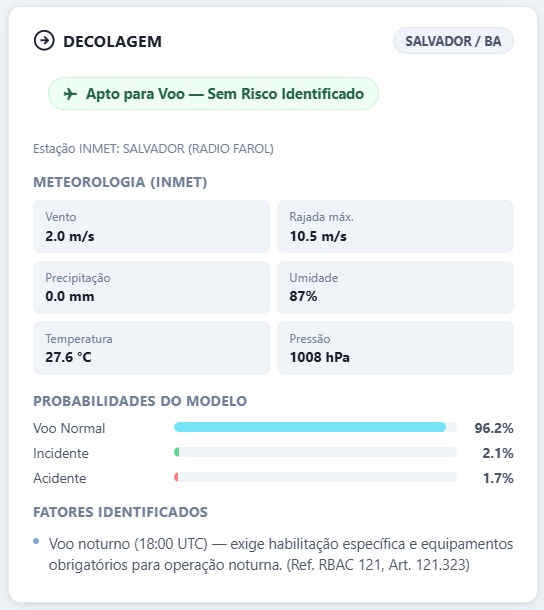
\includegraphics[width=0.85\textwidth]{images/Exemplo_apto_seguro.png}
  \caption{Interface do sistema: status \textbf{Apto Seguro} (Classe 0, confiança $\geq$ 90\%)}
  \label{fig:apto_seguro}
  \fonte{Elaborado pelo autor.}
\end{figure}

\begin{figure}[ht]
  \centering
  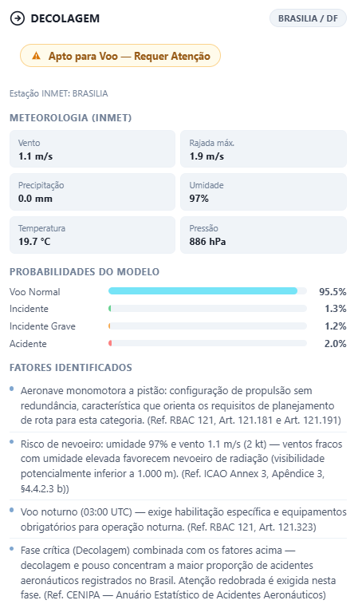
\includegraphics[width=0.85\textwidth]{images/Exemplo_apto_requer_atencao.png}
  \caption{Interface do sistema: status \textbf{Apto Requer Atenção} (condição L1 ativa ou Classe 1)}
  \label{fig:apto_requer}
  \fonte{Elaborado pelo autor.}
\end{figure}

\begin{figure}[ht]
  \centering
  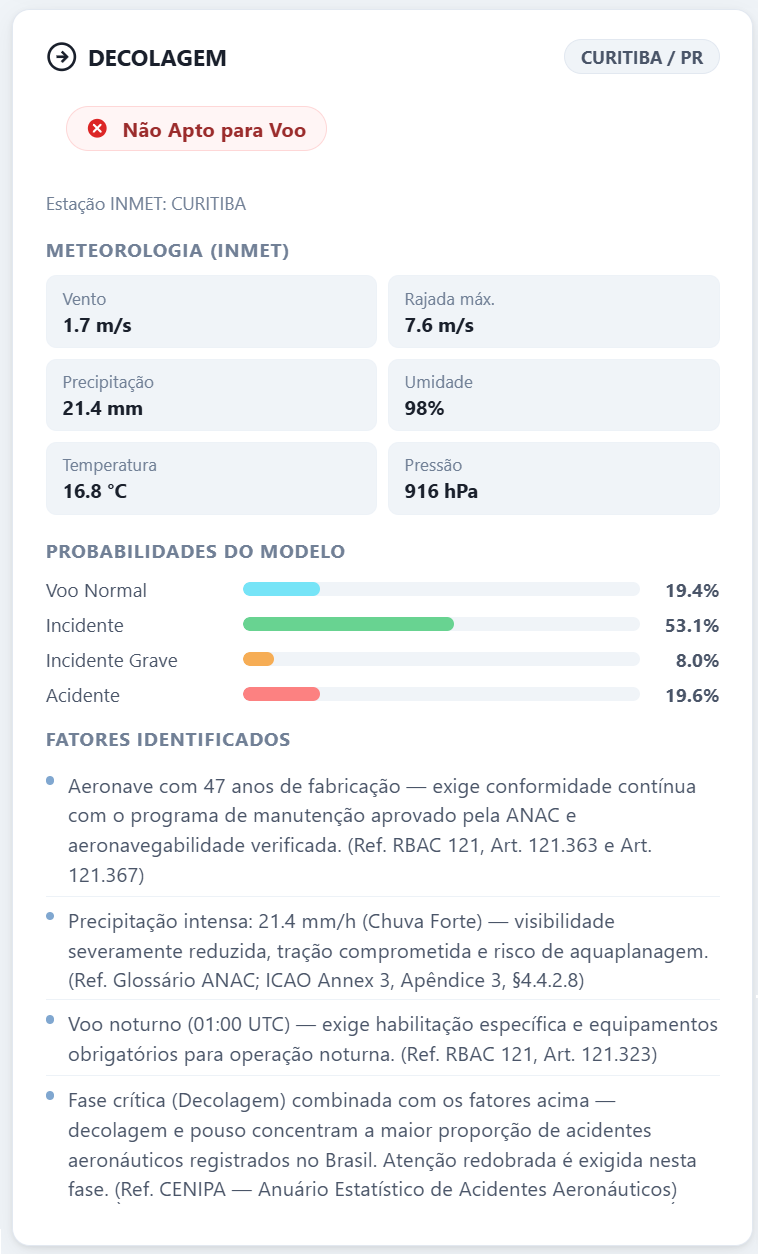
\includegraphics[width=0.85\textwidth]{images/Exemplo_nao_apto.png}
  \caption{Interface do sistema: status \textbf{Não Apto} (condição L2 ativa, Classe 2 ou Classe 3)}
  \label{fig:nao_apto}
  \fonte{Elaborado pelo autor.}
\end{figure}

\begin{figure}[ht]
  \centering
  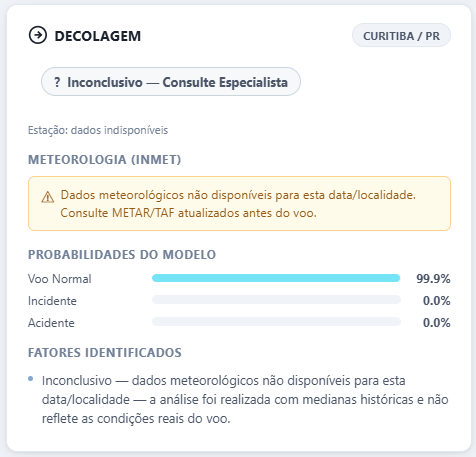
\includegraphics[width=0.85\textwidth]{images/Exemplo_inconclusivo.png}
  \caption{Interface do sistema: status \textbf{Inconclusivo} (baixa confiança ou contradição meteorológica detectada)}
  \label{fig:inconclusivo}
  \fonte{Elaborado pelo autor.}
\end{figure}

\end{document}
